\documentclass[12pt,a4paper,oneside]{article}
\usepackage{amsmath,amsthm}
\usepackage{graphicx}
\usepackage{ctex}
\usepackage{float}
\usepackage{subfigure,subcaption}
\usepackage{caption}
\usepackage{geometry}

\geometry{a4paper,scale=0.8}

\title{计算方法编程作业5实验报告}
\author{张博厚 PB22071354}
\date{}

\begin{document}
\maketitle

\section{实验目的}
对于给定的21个点,实现三次样条插值算法,利用大M法和自然边界条件计算样条插值函数。

\section{问题描述与算法}
\subsection{求解结点处的二阶导数}
由书中公式,可知在自然边界条件下,应求解如下方程:
\begin{figure}[H]
    \centering
    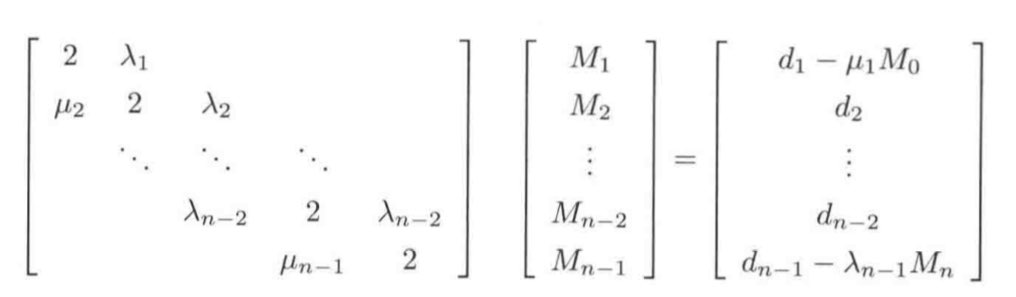
\includegraphics[scale = 0.4]{figs/algo.jpg}
    \caption{待解方程组}
\end{figure}
此处$\lambda_i = \mu_i = 0.5,\ h = 1, 
d_i = \dfrac{6}{h_i+h_{i-1}}(\dfrac{y_{i+1}-y_i}{h_i}-\dfrac{y_i-y_{i-1}}{h_{i-1}})
    = 3(y_{i+1} - 2y_i + y_{i-1})$\\

在本次实验中,选择复用lab2中代码,使用Gauss-Seidel迭代算法来求解上述线性方程组。

\subsection{通过M求解多项式S}
由教材P42公式,有

\begin{align*}
    S(x) &= \dfrac{(x_{i+1}-x)^3M_i+(x-x_i)^3M_{i+1}}{6h_i}+\dfrac{(x_{i+1}-x)y_i-(x-x_i)y_{i+1}}{h_i}-\dfrac{h_i}{6}[(x_{i+1}-x)M_i + (x-x_i)M_{i+1}] \\
         &= \dfrac{M_{i+1}-M_i}{6h}x^3 + \dfrac{M_ix_{i+1}-M_{i+1}x_i}{2h}x^2 + [\dfrac{M_{i+1}x_i^2-M_ix_{i+1}^2+2(y_{i+1}-y_i)}{2h}-\dfrac{h}{6}(M_{i+1}-M_i)]x\\
            &\quad + \dfrac{M_ix_{i+1}^3 - M_{i+1}x_i^3}{6h}+\dfrac{x_{i+1}y_i-x_iy_{i+1}}{h} -\dfrac{h}{6}(M_ix_{i+1}-M_{i+1}x_i)
\end{align*}
代入计算即可得到多项式系数

\section{实验结果与可视化}
对初始数据进行三次样条插值,结果如下:
\begin{figure}[H]
    \centering
    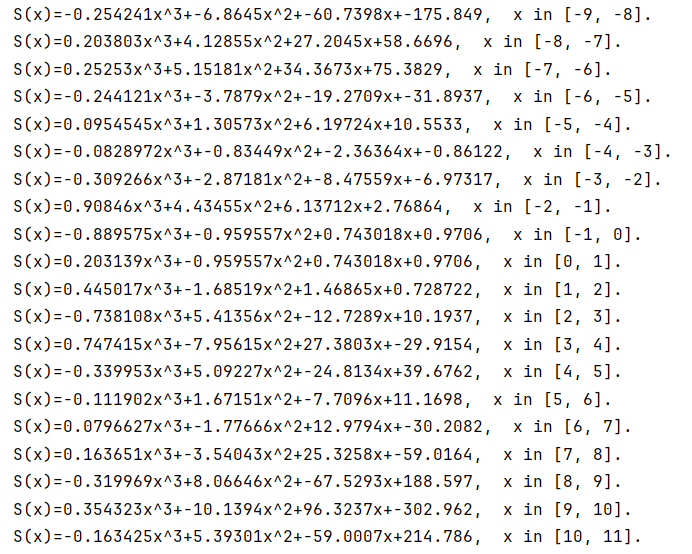
\includegraphics[scale = 0.8]{figs/res1.png}
    \caption{初始数据结果}
\end{figure}
更改第十个点的坐标为(0,10), 再次进行插值得
\begin{figure}[H]
    \centering
    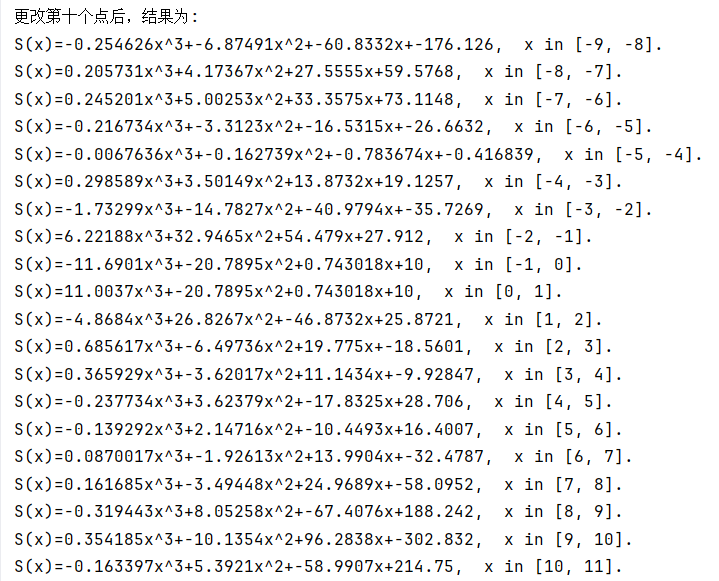
\includegraphics[scale = 0.8]{figs/res2.png}
    \caption{更改点后插值结果}
\end{figure}
分别对前后两次插值结果作比较,计算其系数各自的差,得:
\begin{figure}[H]
    \centering
    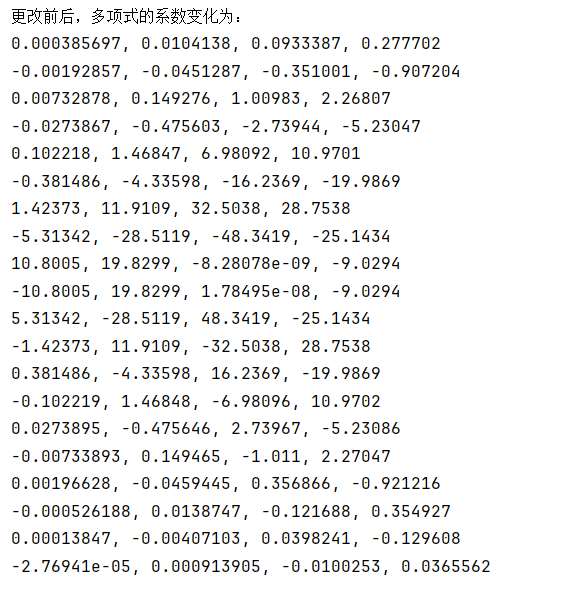
\includegraphics[scale = 0.8]{figs/comp.png}
    \caption{前后结果比较}
\end{figure}
使用Python+matplotlib进行数据可视化,结果如下:
\begin{figure}[H]
    \centering
    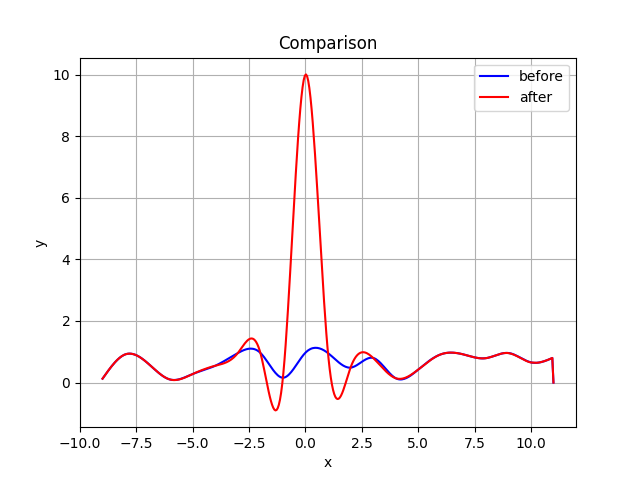
\includegraphics[scale = 0.7]{figs/myplot.png}
    \caption{可视化结果}
\end{figure}
可见,函数仅在更改坐标的点附近变化较大,在其他区间变动几乎可以忽略不计。

\section{实验总结}
综合以上实验结果可以看出,三次样条插值具有良好的连续性和数值稳定性,可以有效
缓解Runge现象,局部数据点的变化不会对较远处的插值函数产生显著影响,是一种强大而灵活的插值方法。


\end{document}